\documentclass[12pt]{article}
\usepackage{amsmath, enumerate, graphicx}
\title{Introduction to Scientific Computation Final Project: Application of MATLAB in analyzing stock price movements through Technical Analysis}
\author{Yohanes Santoso, Abhirup Das, Makensley Lordeus}
\begin{document}
\maketitle

\section{Introduction} 
\hspace{6 mm} Technical Analysis is a branch of study that many investors apply when making decisions regarding purchasing, holding, or selling stocks based on their daily price movements in the market. In contrast to conventional methods of analysis, Technical Analysis fails to recognize the value of the company as a key indicator, and focuses heavily on signals that are directed through the daily and possibly volatile stock price movements in the market. Relying heavily on historical prices, technical analysts assess different indicators through plotting the available data as charts, and aim to make their investment decisions by observing the price, trend or direction of the stock movements. There are several tools to study the applications of technical analysis. However, before proceeding further it is absolutely imperative to lay down the assumptions that govern the study of technical analysis:
\begin{enumerate}[(a)] 
\item Stock Prices tend to move in trends
\item Price movements are seen to be repetitive or cyclical in nature
\item Price movements are a function of the supply and demand of a particular stock
\item Markets capture all characteristics of the traded firms, reflected by the prices
\end{enumerate}
\hspace{6 mm}In our paper, we use four different tools of Technical Analysis in order to chart and assess investment decisions. They are as follows:
\begin{enumerate}[(a)]
\item Moving Average Convergence Divergence (macd)
\item Williams R
\item Relative Strength Index (rsi)
\item Bollinger Bands
\end{enumerate}
\hspace{6 mm}MATLAB allows us to analyze such trends through the use of the Financial Toolbox, and our paper aims to explore the methods of its application and finally complement our findings with the help of examples.

\section{Moving Average Convergence Divergence}
\hspace{6 mm}The MACD is a key resource for most technical analysts. It is commonly grouped under a technical oscillator that serves as an indication to buy or sell a stock, when an overbought or oversold condition is occurring, and defining the end of a trend. It incorporates moving averages that act as lagged indicators to portray trends or characteristics.

Usually MACD is calculated as the difference between the security’s 26 day and 12 day exponential moving averages of the closing price (EMA). Shorter the time period, faster the exponential moving average and vice versa. Nonetheless, a 9 day EMA is plotted alongside the MACD that acts as signal line. Charting the two lines generate trading signals that indicate:
\begin{enumerate}[(a)] 
\item Bullish crossover when MACD moves above the 9-day EMA – Buy
\item Bearish crossover when MACD moves below the 9-day EMA – Sell 
\end{enumerate}
Based on the graph we can therefore analyze the trend when to buy or sell, and hence realize great gains in the market through the application of this knowledge.

In our example, we gathered the stock price information of IBM between the time periods of 1st January 2010 to 1st May 2011 for the short term and 1st May, 2009 to 1st May 2011 to capture the longer time period. The MACD and the 9 day EMA was then calculated using MATLAB. The financial toolbox lets us calculate these values using the function macd. The values were then charted on the graph accordingly. 

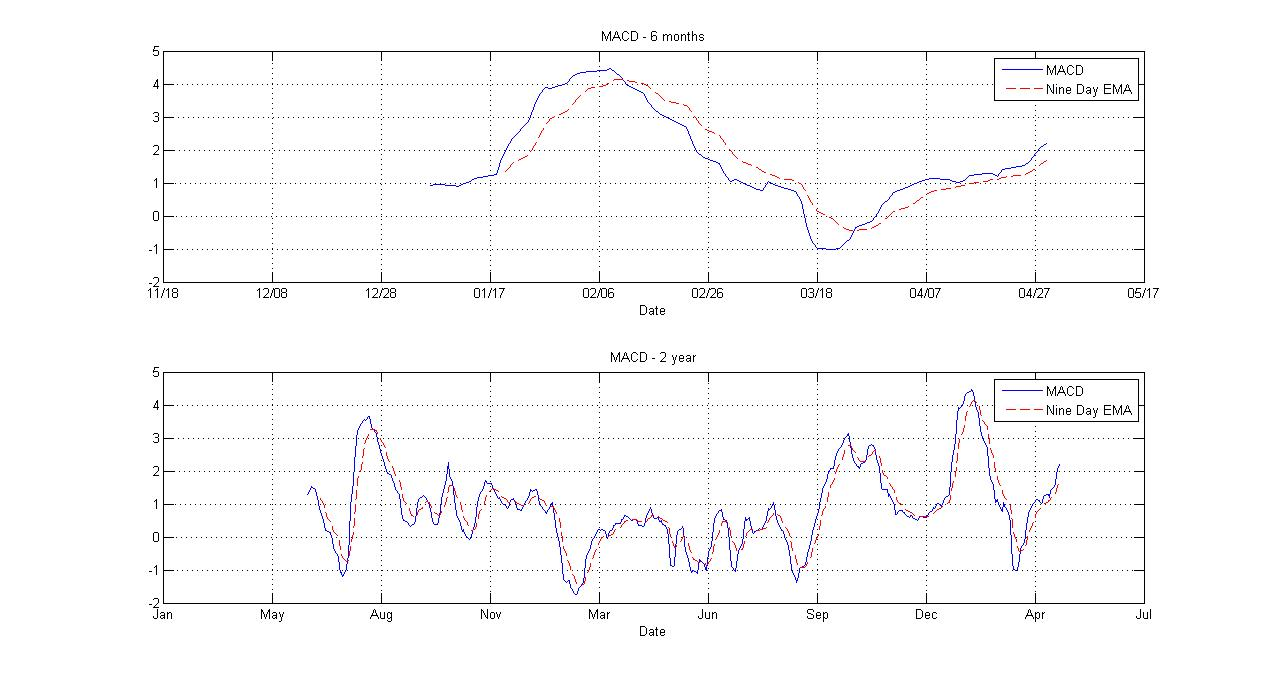
\includegraphics[height=4in,width=5.5in]{MACD.jpg}

The red dotted line represents the nine day EMA, while the blue line represents our MACD line. When checking for the 6 month period, we observe that it was advisable to sell after 26th Feb, and buy after 18th March. We also observe that the NEMA and the MACD are both increasing at the end of the data – hence giving no information regarding buying or selling. Similarly, the 2 year analysis also signals buying and selling points, with the latest being a strong bullish indication to buy the stocks.

\section{Relative Strength Index}
\hspace{6 mm}The RSI is another technical indicator that is used to compare the magnitude of recent gains over recent losses in an attempt to capture overbought or oversold conditions in the market. Incorporating the daily closing prices, the RSI is used as a momentum oscillator that measures the velocity of the directional price movements. Here, momentum is defined as the rate of the rise in prices or the rate of fall in stock prices. Conventionally, a time period of 14 days is used to calculate the RSI. However, many analysts use a variety of time periods in order to capture the RSI effect over a horizon of time.

Nevertheless, for each trading period the gains and losses are calculated. If we observe an upward movement of the closing prices, then the gains are calculated as:
\[
		Gain=Price_{t}-Price_{t-1}
\]
\[
		Loss=0
\] 

Conversely, if the closing prices fall then the losses are calculated as:
\[
		Gain=0
\]
\[
		Loss=Price_{t}-Price_{t-1}
\]

The average gains and losses are then used to calculate the Relative Strength (RS) and the Relative Strength Index (RSI) given by:
\[
		\frac{RS=EMA(Gain, n)}{EMA(Loss, n)} \text{ ; where n = time period}
\]
\[
		RSI=1- \frac{100}{RS}
\]

The RSI is measured from a scale of 0 to 100, with 30 and 70 marking the low and high levels. Once the RSI approaches 70, the security is considered to be overbought indicating a possibility of overvaluation and therefore a good time to sell. Similarly, a value of 30 marks that the security is oversold, indicating that it may be undervalued and hence a great time to buy. For instance, an analyst would recommend selling your IBM stock as of May 1st 2011, because the RSI graph portrays that IBM is being overbought. The results are consistent over both the short term and the long term horizon.  

\graphicspath{{C:\Users\Santosoy\Downloads}}
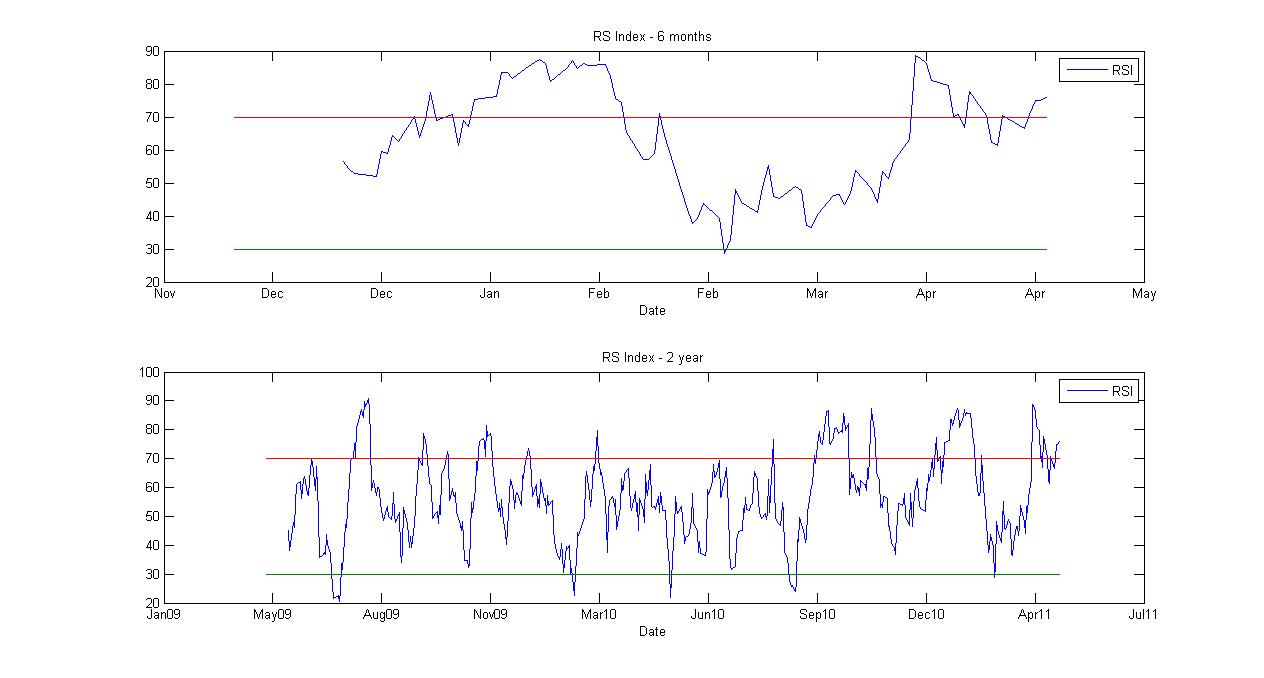
\includegraphics[height=4in,width=5.5in]{RSI.jpg}

\subsection{Notes}
\hspace{6 mm}In order to understand some of the equations above, you may need the following formulas.
\[
		EMA=Price_{t}*K+EMA_{t-1}*(1-K)
\]
\[
    K=\text{ Smoothing Constant }=\frac{2}{(1+N)}
\]
\[
		N=\text{ Number of days in EMA}
\]

The exponential moving averages should be appropriately initialized with simple averages using the first n values in the price series.

\section{Williams \%R}
\hspace{6 mm}William's \%R is a momentum oscillator that tells whether a stock is at a relatively high point in its trading range. It compares the current close of a stock with the high that occurred during the time window. Williams's \%R is usually calculated for a 14 periods (days, weeks, months, or intraday).The formula for the Williams \%R is:
\[
		\%R=[\frac{H-C}{H-L}]*(-100)
\]

Where H is the highest high for period, C is the most recent close, and L is the low. The Williams \%R produces values that oscillate from 0 to -100. Low readings indicates that the price is near its low for the given time period. High readings indicate that the price is near its high for the given time period. It is easy to identify overbought and oversold levels, since Williams \%R is a bound oscillator. The Williams \%R will always fluctuate within this range, no matter how volatile a stock is. Stocks from 0 to -20 are considered overbought and stocks from -80 to -100 are considered oversold.

The Matlab Financial Toolbox has a built in function for calculating Williams \%R:
\[
		wpctr=willpctr(highp, lowp, closep, nperiods)
\]

Highp is a vector containing H, lowp is a vector containing L, closep is a vector containing C, and nperiods is scalar that represent the number of periods that you calculate for (if left blank, the default value is 14). It returns a vector that contains the Williams \%R, which could be charted by plotting it against the time vector of the original data set.
Using the price history for Apple, we are able to get the Williams \%R for the past year, Figure 1. The Chart shows that Apple reached an oversold position in August 2010 and April 2011. It also shows that Apple was overbought between September 2010 and January 2011. When the stock is oversold, you would want to buy it when it Williams \%R indicator moves back above the 80\% mark. When the stock is overbought, you would want to sell when it starts to move pass the 20\% mark.

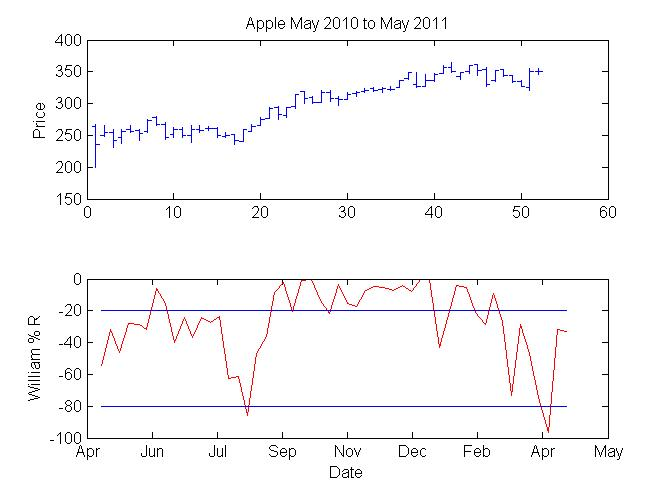
\includegraphics[height=4in,width=5.5in]{apple.jpg}

\section{Bollinger Bands}
\hspace{6 mm}Bands envelope around a moving average but are calculated to adjust for the price volatility around the moving average. They used to find entry position for high probability of profit. To construct Bollinger Bands, you need to calculate a simple moving average of prices (SMA). Then draw bands a certain number of standard deviations above and below the moving average. For example, Bollinger's standard calculation, and the most often seen in the public chart services, begins with a 20-period simple moving average. Two standard deviations are added to the SMA to plot an upper band. The lower band is constructed by subtracting two standard deviations from the SMA. The bands are self-adjusting, automatically becoming wider during periods of extreme price changes.

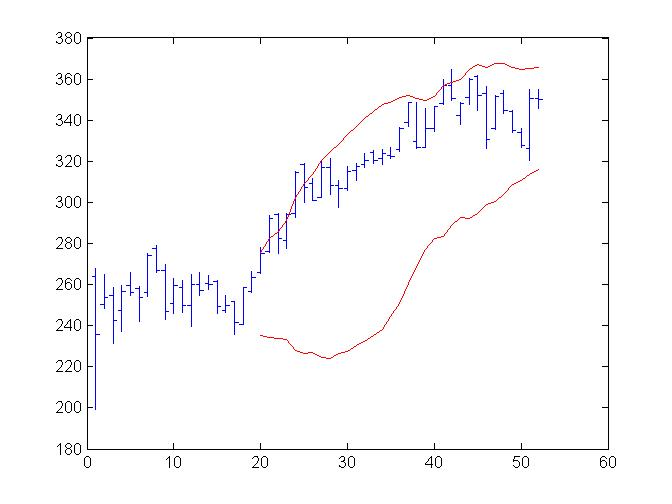
\includegraphics[height=4in,width=5.5in]{bollinger.jpg}

Theoretically, the plus or minus two standard deviations should account for approximately 95\% of all the price action about the moving average. This is not accurate because price action is no stationary and nonrandom and, thus, doesn't follow the statistical properties of the standard deviation calculation precisely. However, it is a good estimate of the majority of price action. The price action seems to oscillate between the bands quite regularly. The moving average is replicating the trend of the prices and adjusting for them while the band is describing their normal upper and lower limits around the trend as price volatility changes.

Bollinger bands could be calculated using Matlabs Financial Toolbox's function:
\[
		[mid, uppr, lowr]=bollinger(data, wsize, wts, nstd)
\]

Data is the data vector, wsize is the window size (optional, the default is 20), wts is the weight factor (0 is box and 1 is linear), and nstd is the number of standard deviations for upper and lower bands (optional, 2 is the default). It returns a vector with the SMA, upper band, and lower band.










\begin{thebibliography}{9}


\bibitem{Erdos01} P. Erd\H os,
\emph{A selection of problems and results in combinatorics},
Recent trends in combinatorics (Matrahaza, 1995),
Cambridge Univ. Press, Cambridge, 2001, pp. 1--6.

\bibitem{ConcreteMath}
R.L. Graham, D.E. Knuth, and O. Patashnik,
\emph{Concrete mathematics}, Addison-Wesley, Reading, MA, 1989.

\bibitem{Knuth92} D.E. Knuth,
\emph{Two notes on notation}, Amer.
Math. Monthly \textbf{99} (1992), 403--422.

\bibitem{Simpson} H. Simpson,
\emph{Proof of the Riemann Hypothesis},
preprint (2003), available at
{\tt http://www.math.drofnats.edu/riemann.ps}.

\end{thebibliography}
 \end{document}
